\label{chap.6}
\section{Forecasting Objective}
\label{sec:forecasting_objective}
The forecasting stage predicts the demand of every cell for the next ten minutes, separately for the three slices, using the recent history of the cell and of its neighbours. In the unified environment (Chapter~\ref{chap.4}) the prediction is a vector of three numbers in Mbps per cell. The earlier B5G and NeversNet5G experiments used a similar network to predict throughput, latency and load. A softplus kept the first two non-negative, and a sigmoid kept the load between 0 and 1.

\section{Graph Construction Across Datasets}
\label{sec:graph_construction}
The implementation supports three graph sources.
\paragraph{Milan grid.} The traffic lies on a regular $100\times100$ grid. Each cell is a node joined to its four neighbours, so the graph is the real geographic neighbourhood. The first experiments used a central $20\times20$ block of 400 cells. The final forecaster covers all 10{,}000 cells.
\paragraph{NeversNet5G.} Here the graph snapshots come from event-driven UE telemetry and keep the identities of the UEs and gNodeBs and how they relate over time. The 64-dimensional SSL embeddings we exported are aligned with the graph timestamps. When a gNodeB has no embedding of its own, we average the embeddings of the UEs connected to it.
\paragraph{B5G topology.} The B5G pipeline uses the graph, the routing matrix and the slice configuration that come with the dataset. It replays recorded samples instead of running an online simulator, and the recorded delta value serves as the reward.

\section{GraphSAGE--GRU Architecture}
\label{sec:graphsage_gru}
At every time step two GraphSAGE layers combine each node's features with the mean of its neighbours' features,
\begin{equation}
h_v^{(l+1)} = \sigma\!\left(W^{(l)}\left[h_v^{(l)} \,\Vert\, \operatorname{mean}_{u\in\mathcal{N}(v)} h_u^{(l)}\right]\right),
\label{eq:graphsage_update}
\end{equation}
where $h_v^{(l)}$ is the representation of node $v$ at layer $l$, $\mathcal{N}(v)$ its neighbours, $W^{(l)}$ a weight matrix and $\sigma$ an activation \cite{hamilton2017}. The sequence of spatial representations over the observation window is fed to a GRU cell, and the final hidden state is used to predict the next interval. The temporal part is a plain \texttt{GRUCell} over the output of PyTorch Geometric's \texttt{SAGEConv}, not the graph-convolutional GRU of the original design, because \texttt{torch\_sparse} did not install on the Windows development machine.

\section{First Experiments on the Milan Block}
\label{sec:milan_tgnn_experiments}
The first experiment used 400 cells over one day of 144 ten-minute steps, with a window of five steps (111 training and 28 validation windows) and 25 epochs of Adam at a learning rate of 0.0005. We compared the TGNN with persistence and with the training mean.
\begin{table}[htbp]
\centering
\caption{First Milan block experiment (one day, 400 cells, one seed)}
\label{tab:milan_forecasting}
\begin{tabular}{|l|c|}
\hline
\textbf{Model} & \textbf{Validation MSE} \\ \hline
GraphSAGE--GRU TGNN & 0.0006160 \\ \hline
Persistence & 0.0007196 \\ \hline
Training-mean predictor & 0.0063946 \\ \hline
\end{tabular}
\end{table}
The TGNN was about 14\% better than persistence. With only one day and one seed this shows that the model can learn the short-term pattern, not that it generalises. Feeding the five raw features in place of the SSL embeddings gave 0.0006122, so the embedding added nothing (Chapter~\ref{chap.5}).

\begin{figure}[htbp]
\centering
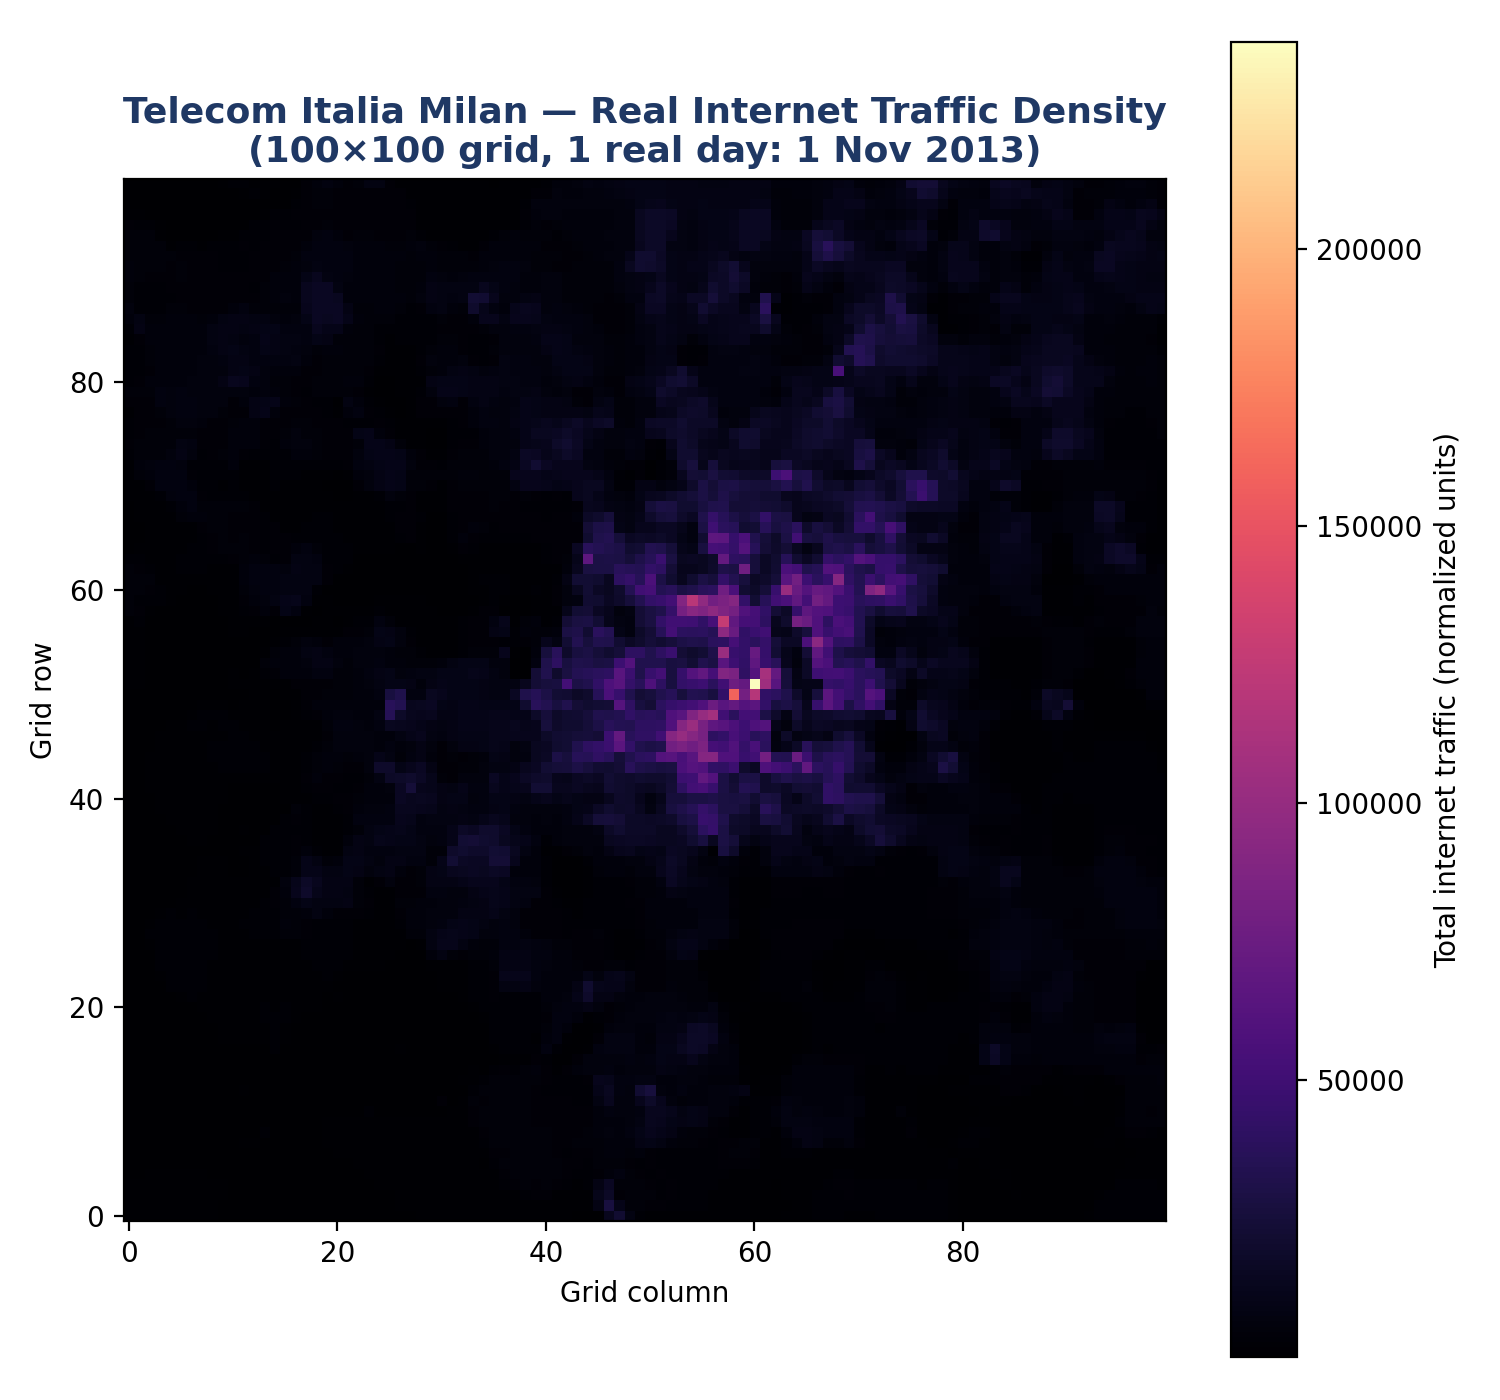
\includegraphics[width=0.55\textwidth,keepaspectratio]{milan_traffic_heatmap.png}
\caption{Real traffic on the Milan grid}
\label{fig:milan_heatmap}
\end{figure}\begin{figure}[htbp]
\centering
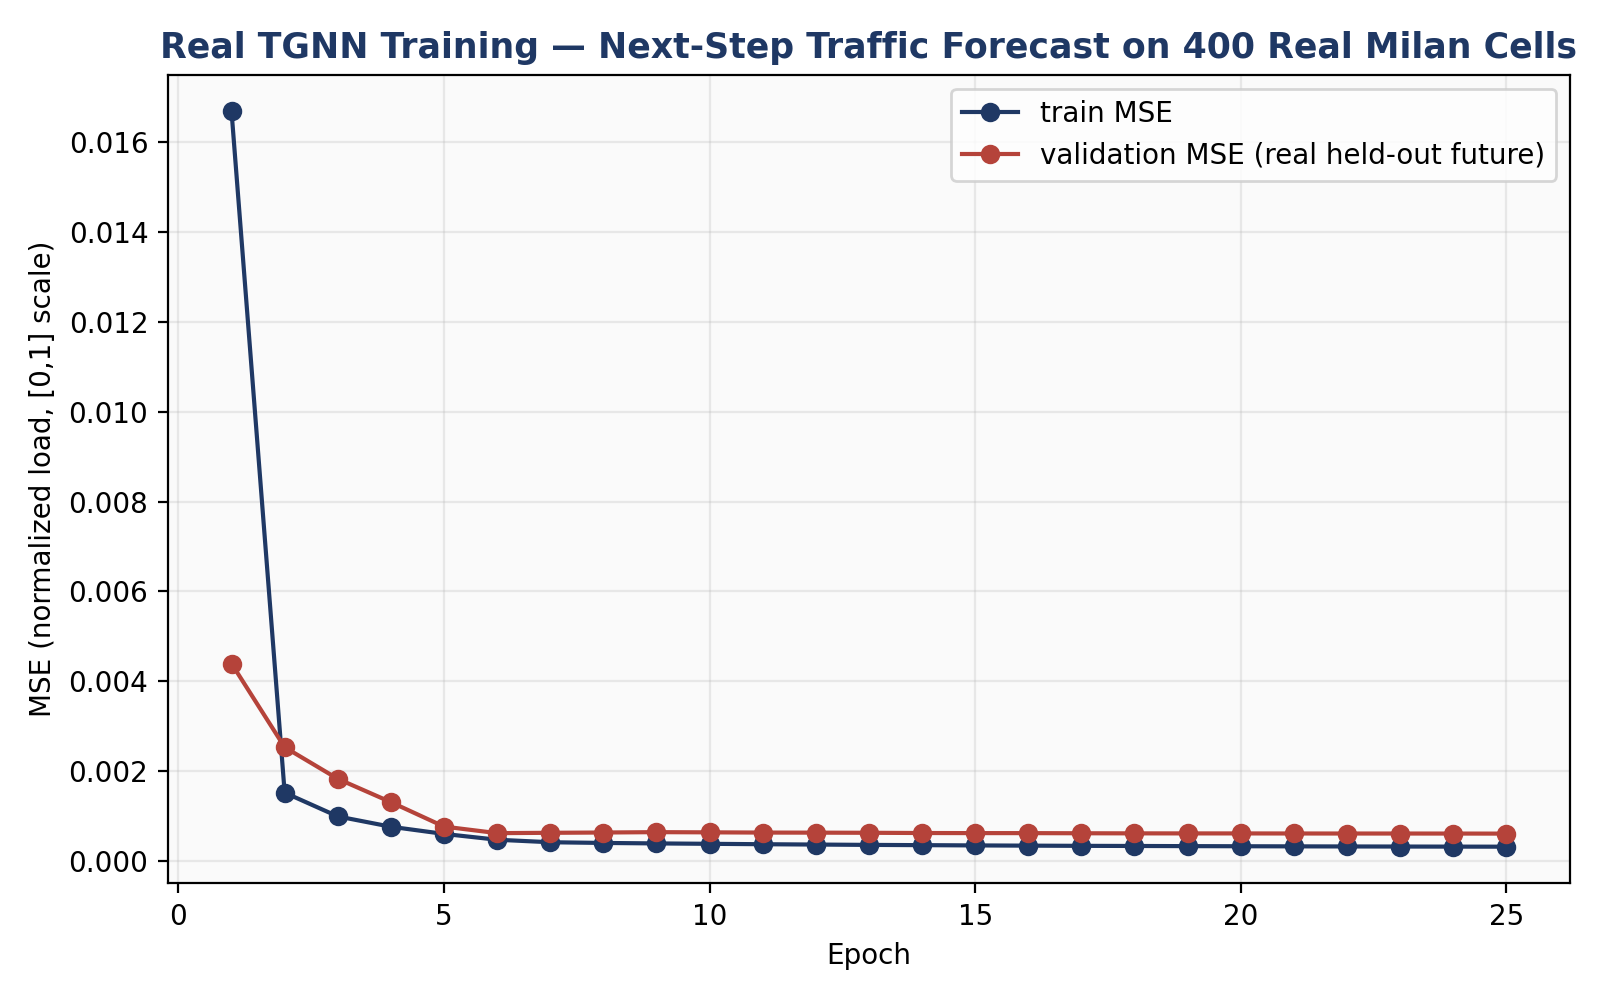
\includegraphics[width=0.8\textwidth,keepaspectratio]{tgnn_milan_forecast_training.png}
\caption{Training and validation error of the first Milan forecaster}
\label{fig:tgnn_first_training}
\end{figure}

\section{City-Wide Generalisation Failure}
\label{sec:city_generalisation_failure}
We applied the forecaster trained on the 100 central cells to all 10{,}000 cells of the city, and it failed on the quiet ones. It had only seen the dense centre, so it had learned that traffic is heavy, and it over-predicted the suburbs by about 6 Mbps on average. On the 9{,}600 outer cells its eMBB error was 10.8 times that of persistence.

\begin{table}[htbp]
\centering
\caption{City-wide evaluation of the forecaster trained on the 100 central cells only (eMBB mean squared error, Mbps$^2$, two held-out days)}
\label{tab:block_city_generalisation}
\footnotesize
\begin{tabular}{|>{\centering\arraybackslash}p{\dimexpr 0.300\textwidth-2\tabcolsep\relax}|>{\centering\arraybackslash}p{\dimexpr 0.170\textwidth-2\tabcolsep\relax}|>{\centering\arraybackslash}p{\dimexpr 0.170\textwidth-2\tabcolsep\relax}|>{\centering\arraybackslash}p{\dimexpr 0.170\textwidth-2\tabcolsep\relax}|}
\hline
\textbf{Region} & \textbf{TGNN} & \textbf{Persistence} & \textbf{TGNN error relative to persistence} \\ \hline
100-cell block & 54.00 & 61.23 & 0.9$\times$ \\ \hline
300-cell core ring & 61.59 & 57.10 & 1.1$\times$ \\ \hline
9{,}600 outer cells & 47.54 & 4.38 & 10.8$\times$ \\ \hline
All 10{,}000 cells & 48.03 & 6.53 & 7.4$\times$ \\ \hline
\end{tabular}
\end{table}

This is a level-bias and spatial-coverage problem: a model that has never seen a quiet cell cannot predict one.

\section{The Corrected City Forecaster}
\label{sec:corrected_city_forecaster}
The architecture was kept and the training was changed in four ways.
\begin{enumerate}
\item \textbf{Per-cell scaling.} We divide the demand of each cell by its own typical level (the median over the training days of its daily 95th percentile, with a floor of 1\% of the city-wide value). The model then learns the shape of the change and not the level.
\item \textbf{Spatial sampling.} Every training step uses a randomly placed $32\times32$ patch of the grid, so central, suburban and intermediate traffic are all seen.
\item \textbf{More data and better inputs.} The model trains on 39 real days. Days 5 and 6 are left out because we use them later for tests, and days 41 to 44 serve as validation for choosing the epoch. Each step also sees the demand of the cell at the same time on the previous day, which is known in advance, plus a time-of-day encoding and a weekend flag.
\item \textbf{No output ceiling.} The old output layer passed the mMTC prediction through a sigmoid, which capped it at the usual level of the cell. The new head predicts a correction to the last observed demand with no upper limit, so spikes can be forecast.
\end{enumerate}
We test the model on a held-out week, 16 to 22 December 2013 (days 45 to 51), over every cell and against persistence. Table~\ref{tab:city_forecaster_improvement} gives the improvement in mean squared error.

\begin{table}[htbp]
\centering
\caption{Improvement over persistence on the held-out week, 16--22 December 2013 (eMBB / URLLC / mMTC)}
\label{tab:city_forecaster_improvement}
\footnotesize
\begin{tabular}{|>{\centering\arraybackslash}p{\dimexpr 0.300\textwidth-2\tabcolsep\relax}|>{\centering\arraybackslash}p{\dimexpr 0.170\textwidth-2\tabcolsep\relax}|>{\centering\arraybackslash}p{\dimexpr 0.170\textwidth-2\tabcolsep\relax}|}
\hline
\textbf{Region} & \textbf{Trained on 5 days} & \textbf{Trained on 39 days} \\ \hline
100-cell block & -12\% / +17\% / +21\% & +21\% / +36\% / +35\% \\ \hline
300-cell core ring & -49\% / +8\% / +7\% & +15\% / +33\% / +32\% \\ \hline
9{,}600 outer cells & -34\% / +9\% / +5\% & +18\% / +34\% / +31\% \\ \hline
All 10{,}000 cells & -34\% / +9\% / +7\% & +18\% / +33\% / +31\% \\ \hline
\end{tabular}
\end{table}

\begin{figure}[htbp]
\centering
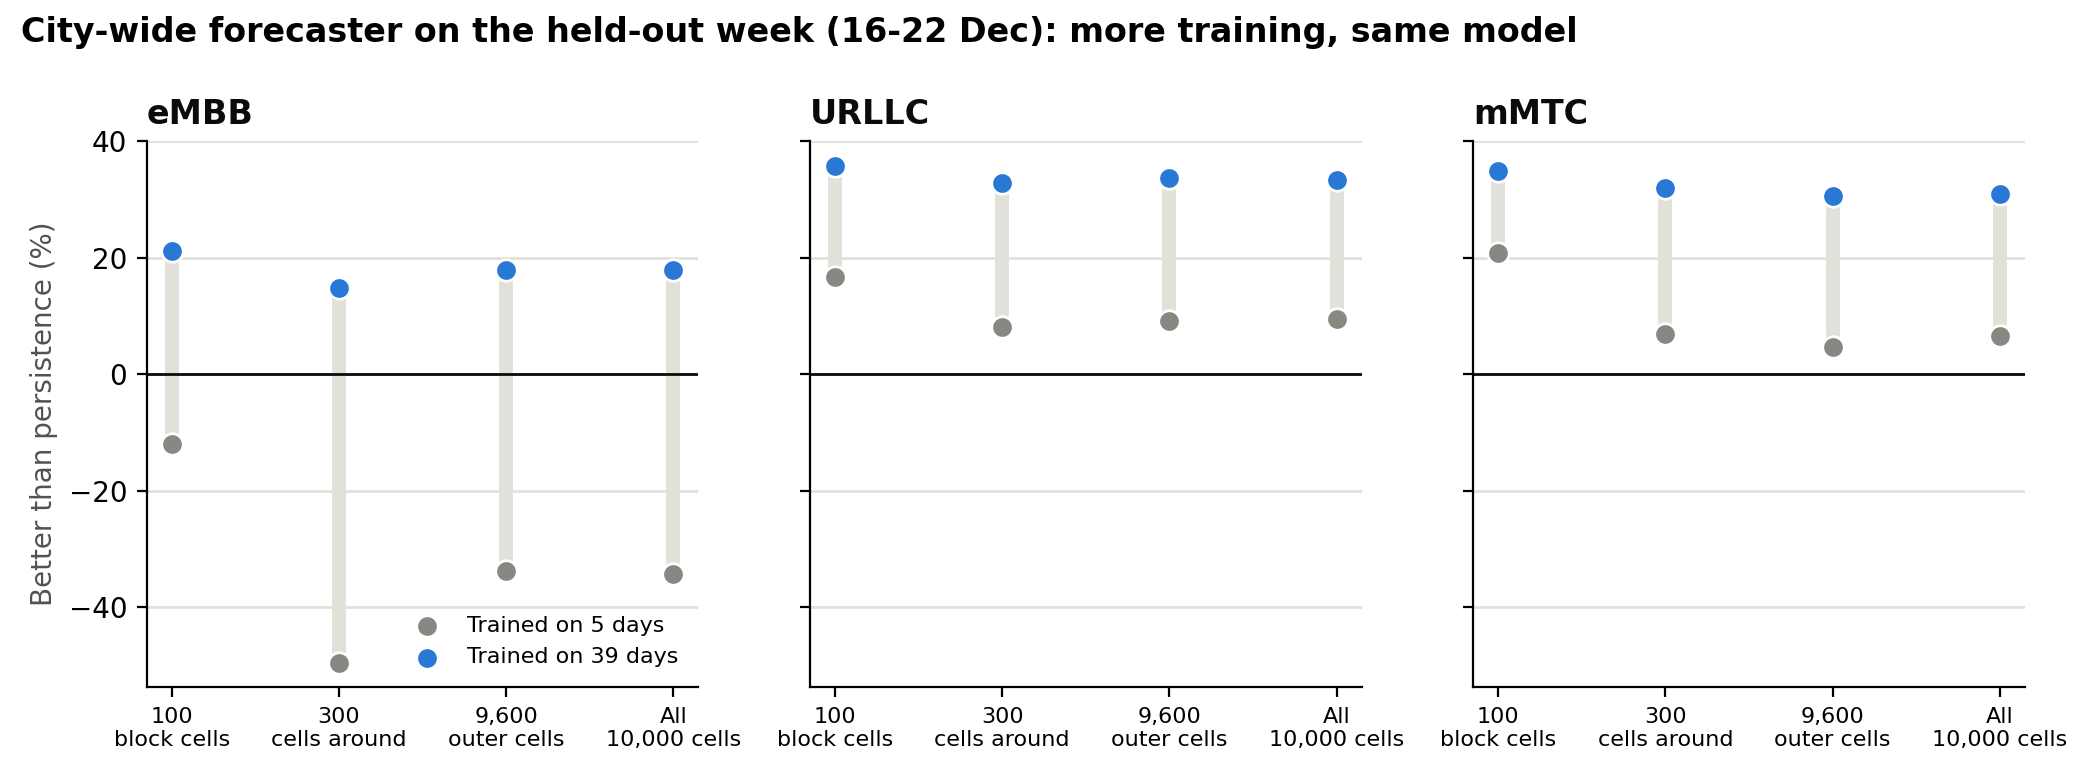
\includegraphics[width=\textwidth,keepaspectratio]{unified_forecast_city.png}
\caption{City-wide forecaster on the held-out week: five days of training against 39 days}
\label{fig:city_forecaster}
\end{figure}

The retrained forecaster beats persistence in every region and for every slice, including the 100 central cells where the earlier model was trained. The five-day version of the same model is worse than persistence on eMBB in this week. So the amount of training data, and not the architecture, was the main limit.

Table~\ref{tab:forecast_baselines} compares the model with two seasonal baselines. At a horizon of ten minutes persistence is very hard to beat. The value at the same time on the previous day gives 8.1 times the eMBB error of persistence, and the average for that time of day gives 13.6 times. Persistence is therefore the right baseline to beat.

\begin{table}[htbp]
\centering
\caption{Mean squared error of simple baselines and the TGNN on all 10{,}000 cells (Mbps$^2$), held-out week}
\label{tab:forecast_baselines}
\footnotesize
\begin{tabular}{|>{\centering\arraybackslash}p{\dimexpr 0.300\textwidth-2\tabcolsep\relax}|>{\centering\arraybackslash}p{\dimexpr 0.170\textwidth-2\tabcolsep\relax}|>{\centering\arraybackslash}p{\dimexpr 0.170\textwidth-2\tabcolsep\relax}|>{\centering\arraybackslash}p{\dimexpr 0.170\textwidth-2\tabcolsep\relax}|}
\hline
\textbf{Forecaster} & \textbf{eMBB} & \textbf{URLLC} & \textbf{mMTC} \\ \hline
Repeat the last value (persistence) & 1.449 & 0.127 & 0.061 \\ \hline
Same time on the previous day & 11.799 & 0.666 & 0.193 \\ \hline
Average for that time of day & 19.736 & 0.522 & 0.152 \\ \hline
TGNN, trained on 39 days & 1.190 & 0.084 & 0.042 \\ \hline
\end{tabular}
\end{table}

\section{Limitations of the Forecasting Study}
\label{sec:pending_forecasting_experiments}
We trained each forecaster once, so we have no estimate of the variation between seeds. We also did not separate the contributions of per-cell scaling, patch sampling, the extra inputs and the graph aggregation, and we have no graph-free baseline (a GRU on each cell alone) or published spatio-temporal baselines such as STGCN. These tests would show which part of the model does the work, and they are listed as future work in Chapter~\ref{chap.10}. The value of the forecast to the controllers is measured in Chapter~\ref{chap.8}.
